%++++++++++++++++++++++++++++++++++++++++
% Don't modify this section unless you know what you're doing!
\documentclass[letterpaper,11pt]{article}
\usepackage{natbib}
\bibliographystyle{unsrtnat}
\usepackage{tabularx} % extra features for tabular environment
\usepackage{amsmath}  % improve math presentation
\usepackage{graphicx} % takes care of graphic including machinery
\usepackage[margin=1in,letterpaper]{geometry} % decreases margins
%\usepackage{cite} % takes care of citations
\usepackage[final]{hyperref} % adds hyper links inside the generated pdf file
\hypersetup{
	colorlinks=true,       % false: boxed links; true: colored links
	linkcolor=blue,        % color of internal links
	citecolor=blue,        % color of links to bibliography
	filecolor=magenta,     % color of file links
	urlcolor=blue         
}
%+++++++++++++++++++++++++++++++++++++++
\begin{document}

\title{NEW GENERATION DATA MODELS AND DBMSS \\\textbf{Fraud Detection (...un titolo figo...)}}
\author{Giussani Riccardo, Cazzetta Davide}
\date{January 2022}
\maketitle

\begin{abstract}
Due righe sul tipo di problema, sul perchè abbiamo scelto mongo; cose belle di Mongo... 
\textbf{ultima cosa da fare}
\end{abstract}

\section{Introduction}
\subsection{Motivation}
\subsection{Conceptual Model}
\begin{enumerate}
    \item ref allo script e due parole sul problema
    \item UML, constraints e supposizioni
\end{enumerate}
explanations, motivations, constraints, and any other information that allows understanding the design carried out.
\\
\begin{figure}[ht] 
        \centering 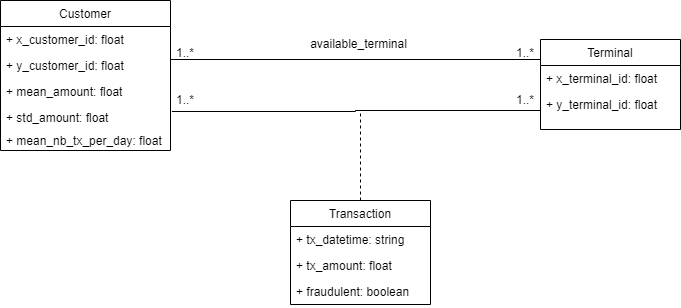
\includegraphics[width=0.9\columnwidth]{images/FraudDetectionUML.png}
        \caption{\label{fig1}Questo è UML dei dati come vengono generati dallo script}
\end{figure}
Come detto ci sono due entità, \textbf{Customer} e \textbf{Terminal}, con la relazione \textbf{Transaction}.
\\
CERCA QUESTIONE ID
\\
Teniamo fissi Customer e Terminal (?)
\\
Tra Customer e Terminal esiste anche la relazione \textbf{available terminal}
\\
In un ipotetico DB relazionale, avrei la tabella \textbf{Transaction} che funge da join table tra Customer e Terminal.
\\
Constraints e supposizioni:
\begin{enumerate}
    \item può sussistere una transaction tra un customer e un terminal se e solo se sussiste tra quei due anche la relazione \textbf{available terminal}
    \item può sussistere la relazione \textbf{available terminal} tra customer e terminal se e solo se il punto in cui si trova terminal è entro un certo raggio dalle coordinate di customer
    \item le coordinate geografiche sono tra 0 e 100
    \item datetime è una stringa conforme
    \item fraudulent è un boolean che dobbiamo calcolare noi
\end{enumerate}

\section{Logical Model}
\subsection{Baseline Model}
Essendo Transactions un'entità centrale, scegliamo di trattarla come entità (nel senso, è una relazione ma è molto importante)\\
\begin{figure}[ht] 
        \centering 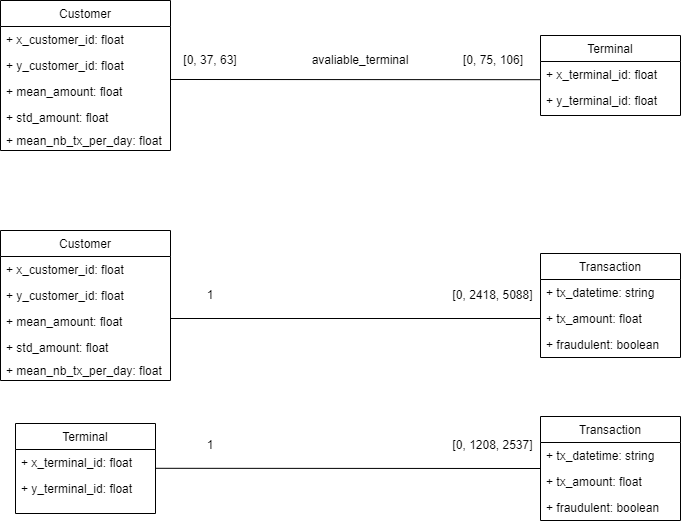
\includegraphics[width=0.9\columnwidth]{images/MongoCardinality.png}
        \caption{\label{fig1}Cardinalità delle relazioni; va bene così perchè card C-T è diversa da quella T-T}
\end{figure}
Queries tell us how we should navigate relationships:
\begin{enumerate}
    \item[a)] requires navigability from Customer to Transaction, to compute the sum
    \item[b)] requires to navigate from terminal to transaction, in order to compute the average, then from transaction to terminal in order to mark fraudulent transactions
    \item[c)] requires to navigate from customer to terminal: we check for customers all terminals used in at least a transaction and then lookup for other customers that allow us to do the chain
    \item[d)] only requires transactions data, and also to generate a new collection, which will navigate from buyingFriends to Customer (we'll see the cardinality). buyingFriends is transitive !
    \item[e)] only requires transactions data
\end{enumerate}
NOTA: i dati di terminal non sono mai acceduti, quindi se ne stanno in una collezione loro e uso solo ref.
\\
The logical data model that has been realized for addressing the requirements imposed by the proposed operations. It is mandatory the presence of the motivations that led to the generation of the data model.
provide a data modeling to optimize the execution of the following operations
\begin{figure}[ht] 
        \centering 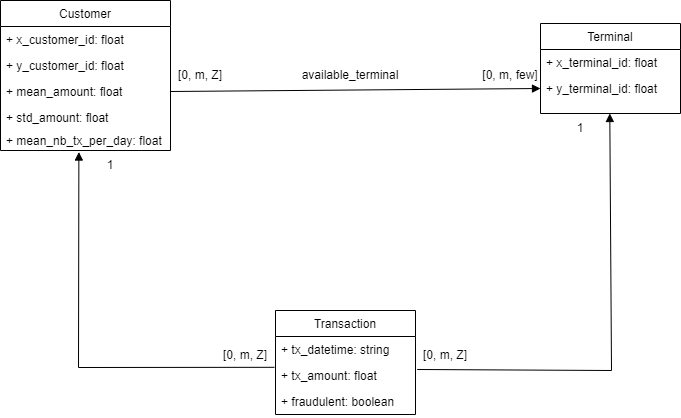
\includegraphics[width=0.9\columnwidth]{images/MongoBaselineNavigability.png}
        \caption{\label{fig1}Questa è la navigabilità baseline, solo guardando le query. Poi bisogna vedere le cardinalità}
\end{figure}
Considerazioni:
\begin{enumerate}
    \item navigation from customer to transaction is impractical: ZILLIONS!
    \item navigation from terminal to transaction is impractical: ZILLIONS!
\end{enumerate}
So we ignore these and just keep navigability from transaction to customer and from transaction to terminal\\
We just navigate from transactions to the other two, do things through a lookup (\textbf{in the baseline case!})
\\
\subsection{Design Patterns}
\textbf{Prima eseguiremo le query sulle collezioni base, poi su quelle ottimizzate coi design pattern per far vedere che si va a migliorare}

\section{Ingestion Layer}
Lo script per mettere i dati su MongoDB\\
Scarichiamo tutte le tabelle. Creiamo file da 50MB / 100MB, ciascuno col suo range di giorni e li andiamo ad aggiungere incrementalmente

\section{Queries}
Come sono implementate le query

\section{Performance}
Valutazione performance, sia nel caso naive che nel caso ottimizzato coi pattern

\section{Conclusion}
This section should be brief, concise, but complete. Directly answer your objectives, state your findings with errors, and conclude whether or not you were successful. Briefly explain if not successful.

\begin{thebibliography}{99}

\bibitem[\protect\citeauthoryear{Author}{2010}]{Author2010}
Author, A.N and Another, A. N., 2010, MNRAS, 431, 28.

\end{thebibliography}

\appendix

\section*{Appendice: Niente}

Prova

\end{document}
